\chapter[Introdução]{Introdução}

\section{Motivação} \label{sec:motivation}

A compreensão acerca do comportamento de sistemas de partículas e de materiais granulados cresceu enormemente nas últimas décadas devido aos esforços da ciência e da engenharia. Tais sistemas são amplamente encontrados em processos industriais e nas ciências naturais \cite{bib:computational_granular_dynamics}, tais como matemática aplicada, física de matéria condensada, geomecânica, agricultura, engenharia química, engenharia civil e engenharia mecânica \cite{bib:rolling}.

Esses conhecimentos são aplicados na previsão do comportamento mecânico de geomateriais, como rochas, e da propagação de trincas e fraturas em sólidos, na simulação da produção de fármacos, alimentos, detergentes e cosméticos, no desenvolvimento de novos materiais e na modelagem da fragmentação, sedimentação, granulação, escavação, transporte e armazenamento de grãos e do escoamento em máquinas extrusoras \cite{bib:donze,bib:poschel,bib:applications}.

\alert{Imagens de aplicações aqui}

% \begin{figure}[h]
% 	\caption{Transporte de grãos}
% 	\vspace{-0.5cm}
% 	\begin{center}
% 		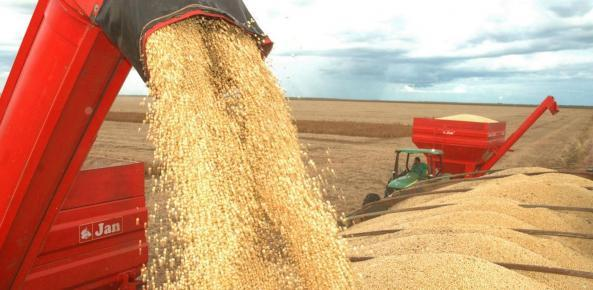
\includegraphics[width=0.6\textwidth]{images/grains_transport.jpg}
% 	\end{center}
% 	% {\centerline{\includegraphics[scale=#2]{#1}}}
% 	\vspace{-0.2cm}
% 	\label{fig:grains_transport}
% 	\legend{Fonte: Confederação da Agricultura e Pecuária do Brasil.\footnote{Disponível em: \url{http://www.cnabrasil.org.br/noticias/pesquisa-vai-quantificar-perdas-no-transporte-de-graos-em-caminhoes}. Acesso em: 04/11/2017}}
% 	% \vspace{-1cm}
% \end{figure}

Sendo assim, surge a necessidade de se compreender a mecânica das partículas.

A análise de sistemas de partículas, contudo, costuma ser bastante complexa. Partículas podem interagir umas com as outras e com o meio em que estão imersas. As interações podem ser forças de contato, forças de corpo, trocas de calor, trocas de carga elétrica, entre outras. Ainda, a quantidade de partículas presentes no sistema de interesse pode facilmente alcançar a ordem dos milhões \cite{bib:computational_granular_dynamics}. Além dessas dificuldades, os problemas estudados geralmente assumem geometrias distintas, tais quais a mistura de substâncias para a produção de fármacos ou o transporte de carga granular.

Com o propósito de executar tais análises, existem três abordagens principais: a experimental, a analítica e a numérica. 

No método experimental, procura-se caracterizar os fenômenos físicos através da sua reprodução em ambientes controlados. A grande vantagem desse método é o fato de lidar com a configuração real do sistema estudado, e dessa análise resultam hipóteses, equações e correlações para as diversas grandezas físicas envolvidas. A experimentação, no entanto, resulta em altíssimo custo e muitas vezes é limitada por questões de segurança ou pela dificuldade de reprodução do sistema real. A experimentação é utilizada para validar modelos físicos e matemáticos \cite{bib:maliska}.

A abordagem analítica, por sua vez, busca a obtenção de soluções analíticas para o problema. A vantagem de se obterem soluções em forma fechada é seu baixíssimo custo de computação quando comparado aos outros métodos. O método analítico, porém, frequentemente depende de hipóteses simplificativas e de geometrias e condições de contorno simples, o que acaba por reduzir a aplicabilidade de seus resultados. Geralmente, utilizam-se soluções analíticas para validar métodos numéricos e auxiliar na busca de métodos mais robustos \cite{bib:maliska}.

A fim de conciliar exatidão e eficiência, os métodos numéricos despontam como uma poderosa ferramenta capaz de resolver problemas complexos, com geometrias complicadas e grande número de partículas, alcançando, apesar disso, uma elevada rapidez e baixíssimo custo \cite{bib:maliska}.

\begin{figure}[h]
	\caption{Comparação entre experimento e simulação de pílulas no interior de um misturador.}
	\vspace{-0.5cm}
	\begin{center}
		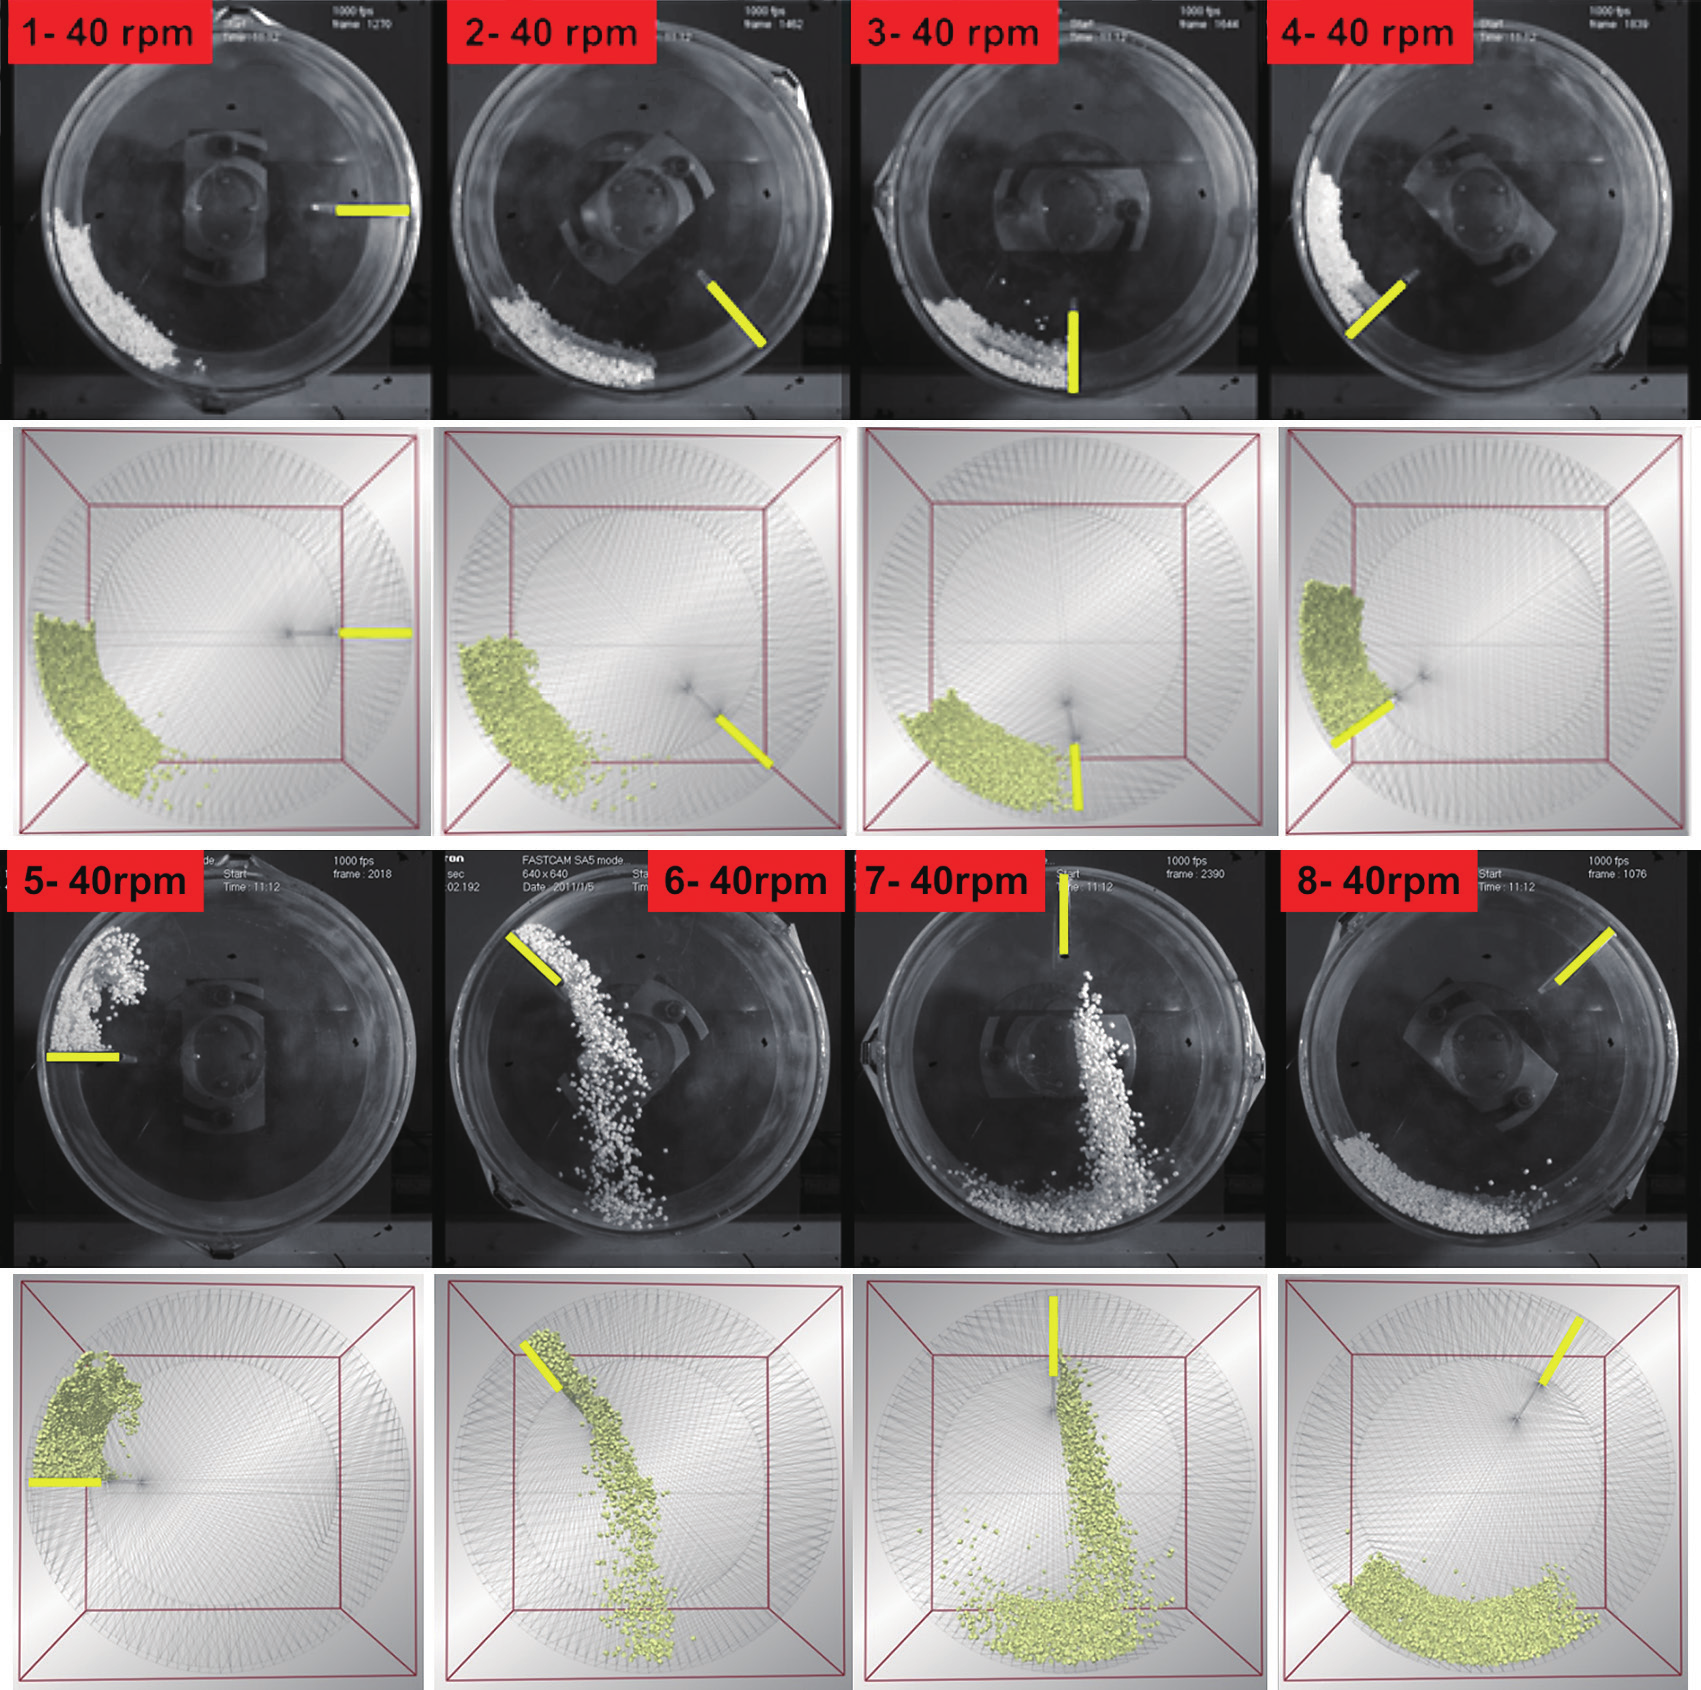
\includegraphics[width=0.65\textwidth]{images/pellet_flow.png}
	\end{center}
	% {\centerline{\includegraphics[scale=#2]{#1}}}
	\vspace{-0.2cm}
	\label{fig:pellet_flow}
	\legend{Fonte: \citeonline{bib:applications}.}
	% \vspace{-1cm}
\end{figure}

\begin{figure}[h]
	\caption{Comparação entre experimento e simulação da mistura de esferas de vidro no interior de um misturador.}
	\vspace{-0.5cm}
	\begin{center}
		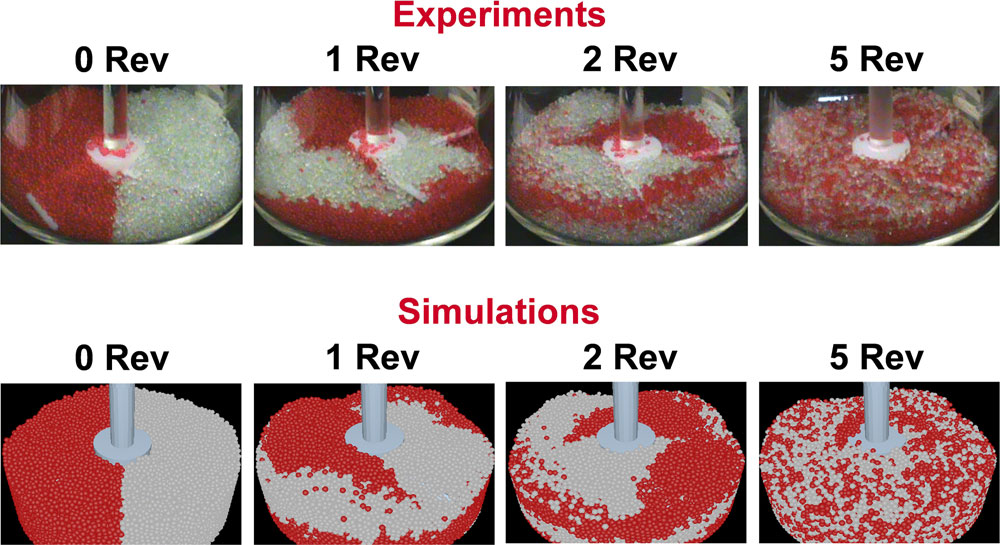
\includegraphics[width=0.65\textwidth]{images/drug_production.png}
	\end{center}
	% {\centerline{\includegraphics[scale=#2]{#1}}}
	\vspace{-0.2cm}
	\label{fig:drug_production}
	\legend{Fonte: \citeonline{bib:future}.}
	\vspace{-1cm}
\end{figure}

As figuras \ref{fig:pellet_flow} e \ref{fig:drug_production} ilustram a capacidade dos métodos numéricos. A primeira delas é uma comparação feita por \citeonline{bib:applications} entre pílulas movendo-se no interior de um tambor rotativo experimentalmente e em uma simulação. A segunda figura representa uma comparação feita por \citeonline{bib:future} entre a mistura de esferas de vidro em um misturador e uma simulação correspondente. As esferas são idênticas a menos de sua cor, que permite uma melhor avaliação dos resultados. Como pode ser observado, embora as simulações não reproduzam \textit{exatamente} a posição das partículas, elas representam com grande fidelidade o sistema estudado.

Sendo assim, o estudo de sistemas de partículas conta principalmente com a simulação numérica como método de análise.
 
\section{Sistemas de Partículas}

A definição de partícula não é um consenso entre autores, cada um adotando o conceito mais adequado à aplicação. Segundo \citeonline{bib:sampaio}, compreende-se por \textit{partícula} um objeto ao qual são atribuídas propriedades físicas, mas cuja estrutura interna é desconsiderada. Cada partícula possui também uma função posição, que descreve a posição de seu centro de massa em função do tempo, e uma função orientação, que determina a posição dos seus eixos principais, sendo que essas duas definições são tomadas com relação a um sistema de referência fixo no espaço.

Por sua vez, um \textit{sistema de partículas} é um conjunto de partículas que interagem entre si. Conforme citado na \autoref{sec:motivation}, essas interações podem ser de diversas naturezas, das quais destacam-se as forças de colisão.

O aspecto dinâmico dos sistemas de partículas é determinado pelas leis de Euler para o movimento:
\begin{gather}
	{\resultingForce}_{,\particle} = \mass_{\particle}\cdot\acceleration_{\particle}, \label{eq:intro_motion_first}\\
	{\resultingTorque}_{,\particle} = \momentOfInertia_{\particle}\deriv{1}{\angularVelocity}_{\particle} + \angularVelocity_{\particle}\cross\pqty{\momentOfInertia_{\particle}\angularVelocity_{\particle}}, \label{eq:intro_motion_second}
\end{gather}
em que \(\position_{\particle}\), \(\angularVelocity_{\particle}\), \(\mass_{\particle}\) e \(\momentOfInertia_{\particle}\) são, respectivamente, a função posição, a função velocidade angular, a massa e o momento de inércia da partícula \(\particle\), enquanto \({\resultingForce}_{,\particle}\) e \({\resultingTorque}_{,\particle}\) são o vetor força resultante e o vetor torque resultante sobre a mesma.

É na solução das equações \eqref{eq:intro_motion_first} e \eqref{eq:intro_motion_second} que consiste a análise acerca dos sistemas de partículas. Essas equações, porém, são de difícil resolução já que a força e o torque resultantes sobre a partícula são oriundas de sua interação com os demais elementos do sistema e são, portanto, funções das propriedades físicas, posições, velocidades, orientações e velocidades angulares dos interagentes.

Em vista disso, é necessário o uso de métodos para a resolução dessas equações, e nessa situação destaca-se o Método dos Elementos Discretos.

\section{O Método dos Elementos Discretos} 

Segundo \citeonline{bib:sampaio}, o Método dos Elementos Discretos, ou DEM (\textit{Discrete Element Method}), refere-se a uma família de métodos computacionais que consideram deslocamentos e rotações de corpos discretos e reconhecem contatos entre elementos automaticamente à medida em que os cálculos são executados. Devido a essa característica, o DEM representa um conjunto de técnicas apropriadas para a simulação do comportamento dinâmico de sistemas de partículas.

Segundo \citeonline{bib:cundall1979}, os cálculos são executados explicitamente, alternando entre a aplicação das leis de Euler para a determinação da posição e da orientação das partículas e a aplicação de relações força-deslocamento para a computação das forças e torques atuantes.

Geralmente, algoritmos de elementos discretos levam em conta a hipótese de partículas rígidas. Uma consequência disso é que, se uma partícula está em contato com outras duas, as interações ocorrem de maneira independente. Com isso, os contatos podem ser computados para cada par de partículas interagentes como se estivessem isoladas das demais.

Cada elemento da simulação pertence a um \textit{tipo}. O tipo de um elemento é usado para determinar a sua geometria e o seu comportamento na simulação. É comum, por exemplo, definir-se um tipo de partícula \textit{fixa}. Partículas desse tipo representam elementos de fronteira, com posição constante e conhecida desde o início da simulação.  

Por sua vez, a geometria das partículas determina quais os modelos de interação que podem ser aplicados. Em geral, o uso de geometrias simples permite a aplicação de modelos também simples, resultando em um custo computacional menor quando comparado às geometrias mais complexas. Certamente, a geometria de partícula necessária depende do sistema que se deseja estudar e do grau de representatividade requisitado. A geometria mais simples é a esférica. Para a obtenção de formas mais complexas, \citeonline{bib:computational_granular_dynamics} apresentam uma técnica de associação de partículas, resultando em \textit{clusters}, com aquele representado na figura \ref{fig:cluster_particle}. \citeonline{bib:computational_granular_dynamics} também tratam de partículas poligonais, enquanto \citeonline{bib:sampaio} demonstra a utilização de superelipsoides.

\begin{figure}[h]
	\caption{Exemplo de associação de partículas simples para a obtenção de geometrias mais complexas.}
	% \vspace{-0.5cm}
	\begin{center}
		\alert{Colocar imagem de uma partícula cluster}
		% 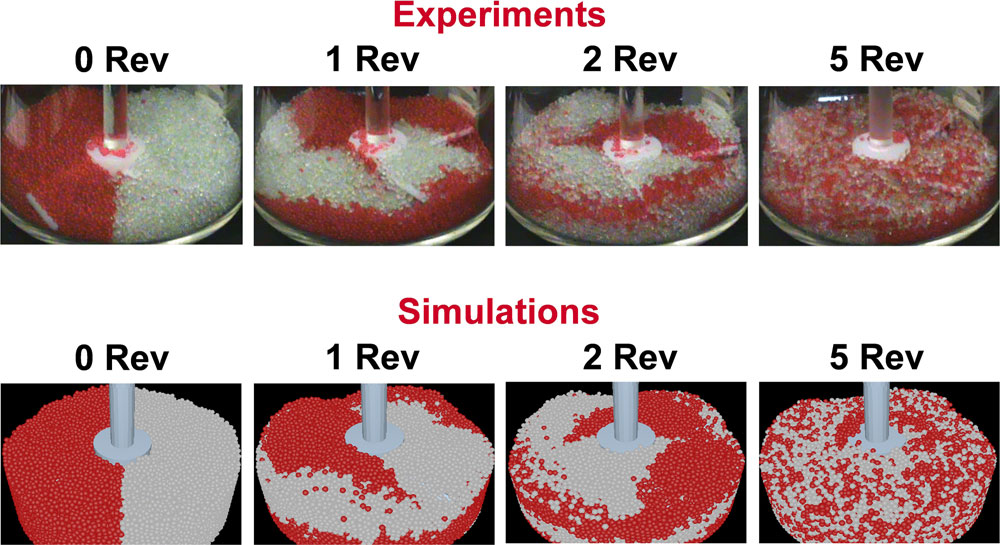
\includegraphics[width=0.65\textwidth]{images/drug_production.png}
	\end{center}
	% {\centerline{\includegraphics[scale=#2]{#1}}}
	% \vspace{-0.2cm}
	\label{fig:cluster_particle}
	\legend{Fonte: \alert{Citar fonte}}
	% \vspace{-1cm}
\end{figure}

O Método de Elementos Discretos é intimamente ligado à Dinâmica Molecular, outra família de métodos computacionais. A distinção que geralmente se faz é que o DEM considera geometrias arbitrariamente complexas, exigindo um tratamento da identificação dos pontos de contato e do cálculo das rotações mais adequado.

Segundo \citeonline{bib:computational_granular_dynamics}, algoritmos do DEM, de forma simplificada, são compostos por algumas etapas principais, sendo elas:
\begin{enumerate}
	\item \textbf{Inicialização:} Nesta etapa, os elementos da simulação são construídos, cada qual com tipo, geometria, propriedades físicas, posição e velocidade iniciais. Também são determinados os modelos de interação considerados e o critério de parada. Esses itens são geralmente definidos por um arquivo de entrada.
	\item \textbf{Predição:} O cálculo de forças e torques atuantes sobre cada partícula depende da posição, da velocidade, da orientação e da velocidade angular dos elementos da simulação, que são desconhecidas no instante futuro. Sendo assim, é necessária uma estimativa, ou \textit{predição}, para os valores dessas variáveis. Essa estimativa é feita na etapa de predição. \label{item:prediction}
	\item \textbf{Interação:} A etapa de interação se divide em duas subetapas:
		\begin{enumerate}
			\item Determinação dos pares de interação. Nem todas as partículas interagem em todos os instantes.
			\item Computação das forças e torques entre os elementos da simulação com base nas coordenadas previstas na etapa \ref{item:prediction}.
		\end{enumerate}
	\item \textbf{Correção:} Nesta etapa, valores corrigidos para as coordenadas (e as respectivas derivadas) das partículas são obtidos através da resolução das equações \eqref{eq:intro_motion_first} e \eqref{eq:intro_motion_second}.
	\item \textbf{Terminação:} Caso o critério de parada previamente estabelecido seja atingido, o programa deve finalizar. Caso contrário, a simulação deve avançar o instante de tempo e retornar ao passo \ref{item:prediction}.
\end{enumerate}

Essas etapas podem ser representadas como na figura \ref{fig:simple_dem_algorithm}. Outros passos podem ser introduzidos no algoritmo, tais quais exportação de dados, iterações em cada passo de tempo e acoplamento com outros simuladores.

\begin{figure}[h]
	\caption{Fluxograma simplificado do Método dos Elementos Discretos.}
	% \vspace{-0.5cm}
	\begin{center}
		\alert{Colocar fluxograma do DEM}
		% 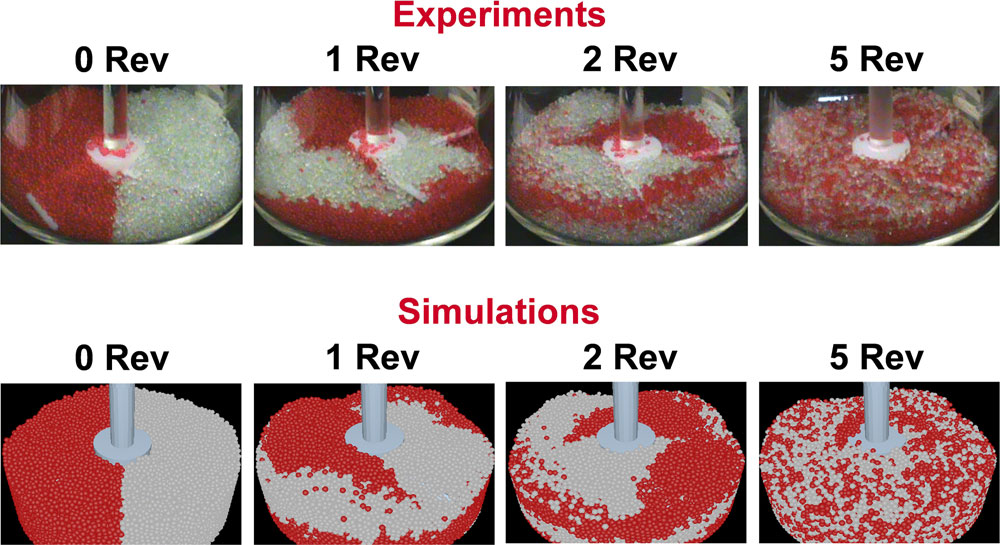
\includegraphics[width=0.65\textwidth]{images/drug_production.png}
	\end{center}
	% {\centerline{\includegraphics[scale=#2]{#1}}}
	% \vspace{-0.2cm}
	\label{fig:simple_dem_algorithm}
	\legend{Fonte: \alert{Citar fonte}}
	% \vspace{-1cm}
\end{figure}

Também é possível acoplar o DEM a outras famílias de métodos, como FEM (Método de Elementos Finitos) e CFD (Fluidodinâmica Computacional). Nesses casos, além das equações de movimento para as partículas, são consideradas equações de conservação de massa, de energia, de carga elétrica, equações de estado, entre outras. Com isso, é possível computar transferência de calor, arraste causado por fluidos e distribuição de tensões em sólidos. \citeonline{bib:donze} e \citeonline{bib:dem_chapter} apresentam alguns exemplos das diversas extensões que podem ser feitas ao DEM. \citeonline{bib:chu_and_yu} explicam e aplicam um modelo para interação entre um fluido e partículas com foco no arrasto, enquanto \citeonline{bib:conductivity} e \citeonline{bib:heat_dem} demonstram a aplicação de modelos de troca de calor. O acoplamento entre DEM e outras famílias é conhecido como EDEM, ou XDEM, o Método de Elementos Discretos Estendido.

\section{Revisão Bibliográfica}

A base matemática para os Métodos de Elementos Discretos foi fundada por Isaac Newton, com a divulgação de suas leis de movimento. Entretanto, devido às dificuldades mencionadas na seção \ref{sec:motivation} tais quais a quantidade de partículas e a natureza das equações diferenciais, a análise de sistemas de partículas só se tornou factível com o advento dos computadores.

O Método dos Elementos Discretos foi primeiramente apresentado por Cundall. Uma descrição do método pode ser encontrada em \citeonline{bib:cundall1979}, em que se consideram atrito e amortecimento na colisão das partículas. A presença de atrito provoca rotações, que devem ser solucionadas juntamente com as posições. Nesse algoritmo, as velocidades eram preditas como constantes durante um passo de tempo.

O método foi ainda extendido com os trabalhos de \citeonline{bib:haff1986}, \apudonline{bib:walton1983}{bib:haff1986}, \citeonline{bib:gallas1992}, além de vários outros.

Dentre as principais referências sobre o DEM, destacam-se \citeonline{bib:liquids}, \citeonline{bib:computational_granular_dynamics} e \citeonline{bib:dem_chapter}.

Além das publicações acadêmicas, existem diversos \textit{softwares} comerciais e de código aberto projetados para simulação com o DEM, cada qual com seus objetivos, vantagens e desvantagens. Dentre os simuladores comerciais, destacam-se o Rocky DEM, o EDEM e o PFD (\textit{Particle Flow Code}). Dentre os principais programas de código aberto estão o Yade, o LIGGGHTS e o KRATOS. Algumas das características desses simuladores são o processamento em paralelo, a capacidade de customização, pós-processamento, geração de scripts, acoplamento entre diferentes físicas, uso de geometrias CAD e acoplamento com outros simuladores.

\section{Objetivos e Contribuições}

O SINMEC - Laboratório de Simulação Numérica em Mecânica dos Fluidos e Transferência de Calor, do Departamento de Engenharia Mecânica da Universidade Federal de Santa Catarina, tem como principal linha de pesquisa a aplicação do método de volumes finitos baseado em elementos (EbFVM) com malhas não estruturadas para a solução de problemas de mecânica de fluidos e transferência de calor.

Devido à importância do tema e à possibilidade de se estudar o acoplamento entre a dinâmica de partículas e os fenômenos de transporte, surgiu o interesse do laboratório em iniciar uma área de pesquisa acerca do Método de Elementos Discretos Estendido utilizando o EbFVM para a solução de escoamentos. Para tanto, porém, é necessária, primeiramente, uma compreensão acerca do DEM.

Sendo assim, este trabalho objetiva iniciar essa linha de pesquisa no SINMEC, desenvolvendo um simulador que seja de fácil extensão, permitindo que novos modelos de interação, tipos de partículas e algoritmos de solução sejam introduzidos à medida que novos estudos sejam feitos. Para que isso se tornasse possível, este trabalho foi subdividido em três partes: primeiramente, uma biblioteca deveria ser implementada, contendo a lógica do funcionamento dos algoritmos DEM, de forma generalizada, sem particularizar suas características; na segunda parte, seria gerado um simulador que, tomando a biblioteca como base, especificasse os tipos de partícula, as interações e os métodos de solução; e, por fim, executar simulações no simulador e validar a implementação através da análise dos resultados e da comparação com soluções analíticas. 
 
Com o propósito de melhor guiar as atividades, são propostos os seguintes objetivos específicos:
\begin{enumerate}
\item Desenvolver uma biblioteca computacional para a simulação da dinâmica de partículas através do DEM. Essa biblioteca deve possuir as seguintes características: \label{item:library}
 	\begin{enumerate}
		\item Suporte para diferentes modelos de colisão, inclusive para modelos estudados e implementados por um usuário posterior;
		\item Capacidade para um número arbitrário de partículas, as quais podem assumir diferentes formas geométricas e possuir várias propriedades físicas;
        \item Permitir a inserção de diferentes tipos de interação entre as partículas. Essas interações podem ter naturezas distintas, como a transferência de calor e a troca de cargas elétricas;
		\item Suporte para variadas funções de busca de partículas vizinhas;
		\item Disponibilidade de utilização de diversos tipos de condição de contorno;
		\item Suporte para diferentes algoritmos de predição e correção;
	\end{enumerate}  
\item Implementar um simulador que, com base na biblioteca desenvolvida, seja capaz de executar simulações que aceitem, no mínimo:
	\begin{enumerate}
		\item Partículas esféricas;
		\item Paredes fixas planas;
		\item Os principais modelos de força de colisão, conforme explicado na seção \ref{sec:collision_force_models};
		\item O algoritmo de Gear, empregando a extrapolação de Taylor, de acordo com o capítulo \ref{ch:mathematical_model};
		\item Simulações em duas dimensões;
	\end{enumerate}
\item Validar a implementação por meio da comparação de resultados de simulações com soluções analíticas para o problema ou através da análise dos resultados.
\end{enumerate}

\section{Organização do Trabalho}

Para melhor cobrir todos os assuntos relativos ao cumprimento dos objetivos, além do capítulo de introdução, este trabalho é dividido nos seguintes capítulos:
\begin{description}
	\item[\autoref{ch:mathematical_model} - \nameref{ch:mathematical_model}:] Nesse capítulo, são abordados os aspectos teóricos e matemáticos concernentes ao DEM. Nele, são descritas as equações de movimento que devem ser solucionadas, alguns dos principais modelos para as forças de colisão e o algoritmo de Gear;
	\item[\autoref{ch:discrete_element_method} - \nameref{ch:discrete_element_method}:] Nesse capítulo, é descrito o DEM, demonstrando como os conceitos apresentados no capítulo \ref{ch:mathematical_model} são aplicados e transformados em algoritmos.
	\item[\autoref{ch:computational_implementation} - \nameref{ch:computational_implementation}:] Esse capítulo evidencia a implementação da biblioteca e do simulador em linguagem C++ ao apresentar códigos, pseudocódigos e fluxogramas com o intuito de fornecer uma visão geral do código e explicar o seu funcionamento.
	\item[\autoref{ch:results} - \nameref{ch:results}:] Esse capítulo é destinado à apresentação de resultados de simulação, à sua confrontação com soluções analíticas e à análise de tais resultados. Com isso, a implementação é validada.
	\item[\autoref{ch:conclusion} - \nameref{ch:conclusion}:] O último capítulo é dedicado a sumarizar o trabalho, reafirmando os principais pontos explorados ao longo do texto e atestando que os objetivos propostos foram alcançados. Também são apresentadas algumas sugestões para trabalhos futuros.
\end{description}